\documentclass{article}
%----------------------------------------------------------------------
\usepackage[polish]{babel}
\usepackage[utf8]{inputenc}
\usepackage[T1]{fontenc}
\usepackage[a4paper,top=2cm,bottom=2cm,left=3cm,right=3cm,marginparwidth=1.75cm]{geometry}
\usepackage{lmodern}
\usepackage{microtype}
\usepackage{amsmath,amssymb}
\usepackage{graphicx}
\usepackage{listings}
\usepackage{etoolbox}
\usepackage{booktabs}
\usepackage{algorithm}
\usepackage[noend]{algpseudocode}
\usepackage{tabularx}
\usepackage{array}
\usepackage{enumitem}
\usepackage[colorlinks=true, linkcolor=black, urlcolor=black, citecolor=black]{hyperref}
\usepackage{csquotes}
\usepackage[backend=biber,style=numeric,sorting=none,maxbibnames=4]{biblatex}
\addbibresource{references.bib}
\usepackage{subcaption}
\usepackage{xcolor}
\usepackage{float}
\usepackage{newfloat}
\usepackage{fancyvrb}
\usepackage{multirow}
\usepackage{siunitx}

% Liczby po polsku: przecinek dziesiętny, spójniki i półpauza w listach i zakresach
\sisetup{
    output-decimal-marker = {,},
    exponent-product = \cdot,
    group-separator = {\,},
    group-minimum-digits = 5,
    uncertainty-mode = separate,
    list-separator = {,~},
    list-pair-separator = {~i~},
    list-final-separator = {~i~},
    range-phrase = {--},
    range-units = single,
}
% Procent bez odstępu, jak na wykresach (94,1%)
\DeclareSIUnit[quantity-product = {}]\percent{\%}

% Wykresy brane wprost z katalogów eksperymentów i badań
\graphicspath{{../data/experiments/}}

% Przełącznik obrazów: \rysunkifalse ukrywa wykresy i diagramy (podpisy i numeracja
% zostają), żeby ocenić objętość samego tekstu. W repozytorium zawsze \rysunkitrue.
\newif\ifrysunki
\rysunkitrue
\ifrysunki\else
    \renewcommand{\includegraphics}[2][]{\mbox{}}
\fi

% Diagramy
\usepackage{tikz}
\usetikzlibrary{positioning, arrows.meta}

% Listingi plików konfiguracyjnych TOML
\lstdefinelanguage{toml}{
    morecomment=[l]{\#},
    morestring=[b]",
    sensitive=true,
}
\lstdefinestyle{config}{
    language=toml,
    basicstyle=\ttfamily\footnotesize,
    commentstyle=\color{consoleGray},
    stringstyle=\color{consoleBlue},
    columns=fullflexible,
    keepspaces=true,
    breaklines=true,
    breakatwhitespace=true,
}
% Proste apostrofy i grawisy w listingach i Verbatim, tak jak w plikach
\usepackage{upquote}

% Definicje kolorów
\definecolor{consoleGreen}{RGB}{22, 198, 12}
\definecolor{consoleRed}{RGB}{197, 15, 31}
\definecolor{consoleYellow}{RGB}{193, 156, 0}
\definecolor{consoleBlue}{RGB}{0, 55, 218}
\definecolor{consoleGray}{RGB}{100, 100, 100}
\definecolor{consolePurple}{RGB}{136, 23, 152}

% Pomocnicze komendy do kolorowania
\newcommand{\txtGreen}[1]{\textcolor{consoleGreen}{#1}}
\newcommand{\txtRed}[1]{\textcolor{consoleRed}{#1}}
\newcommand{\txtYellow}[1]{\textcolor{consoleYellow}{#1}}
\newcommand{\txtBlue}[1]{\textcolor{consoleBlue}{#1}}
\newcommand{\txtGray}[1]{\textcolor{consoleGray}{#1}}
\newcommand{\txtPurple}[1]{\textcolor{consolePurple}{#1}}

\newfloat{code}{H}{loc}[section]
\floatname{code}{Listing}

% Algorytmy po polsku
\floatname{algorithm}{Algorytm}
\renewcommand{\algorithmicrequire}{\textbf{Wejście:}}
\renewcommand{\algorithmicensure}{\textbf{Wyjście:}}

% Oznaczenia używane w tekście
\newcommand{\yhat}{\hat{y}}

\emergencystretch=1.5em

% Sekcje zaczynają się od nowej strony, dopóki nie wyłączymy tego przez \sekcjebezpodzialu
\newif\ifsekcjanowastrona
\sekcjanowastronatrue
\newcommand{\sekcjebezpodzialu}{\sekcjanowastronafalse}
\pretocmd{\section}{\ifsekcjanowastrona\clearpage\fi}{}{}

\lstset{
    basicstyle=\ttfamily, % Ustawienie czcionki monospaced
}

\newcommand{\nazwaprzedmiotu}{Sieci neuronowe}
\newcommand{\tytulprojektu}{Rozpoznawanie cyfr ze zbioru MNIST z~użyciem perceptronu wielowarstwowego}
\newcommand{\nazwadokumentu}{Raport z części drugiej}
\newcommand{\prowadzacy}{dr inż. Maksymilian Bujok \\ mgr inż. Grzegorz Zakrzewski}
%----------------------------------------------------------------------
\begin{document}

\begin{titlepage}
    \centering
    \vspace{1.5cm}
    
\includegraphics[width=0.9\textwidth]{university-logo.png} \\
    \vspace{2.5cm}
    {\fontsize{30}{20}\selectfont \textbf{\nazwaprzedmiotu} \par}
    \vspace{1.5cm}
    {\fontsize{25}{20}\selectfont \tytulprojektu \par}
    \vspace{1.5cm}
    {\fontsize{18}{20}\selectfont \nazwadokumentu \par}
    \vspace{1.5cm}
    {\fontsize{12}{20}\selectfont Zespół: \\ Adam Grącikowski \par}
    \vspace{0.5cm}
    {\fontsize{12}{20}\selectfont Prowadzący: \\ \prowadzacy \par}

    \vfill
    Oświadczam, że niniejsza praca, stanowiąca podstawę do uznania osiągnięcia efektów uczenia się z przedmiotu \textit{\nazwaprzedmiotu}, została wykonana samodzielnie.

    \vspace{1cm}

    Warszawa, \today

\end{titlepage}

%----------------------------------------------------------------------
\section*{Streszczenie}
\phantomsection
\label{sec:abstract}
% Plan (etap 6): użycie sieci z części pierwszej do rozpoznawania cyfr MNIST bez nowych
% funkcjonalności, strojenie jeden-czynnik-naraz na podzbiorze, konfiguracja końcowa,
% dokładność testowa (5 ziaren i zgłoszona sieć).


\tableofcontents
\newpage

%----------------------------------------------------------------------
\section{Wstęp}
\label{sec:introduction}

W rozdziale przedstawiono cel i zakres drugiej części projektu oraz strukturę raportu.

\subsection{Cel i zakres}
\label{sec:introduction-goal}

W pierwszej części projektu zaimplementowano od podstaw, bez bibliotek implementujących sieci neuronowe, perceptron wielowarstwowy uczony propagacją wsteczną błędu i zbadano go w zadaniach regresji i klasyfikacji na prostych zbiorach danych \cite{gracikowski2026}. Celem części drugiej było użycie tej implementacji do rozpoznawania odręcznie pisanych cyfr ze zbioru MNIST \cite{lecun1998}. Implementacji nie wolno było rozszerzać o nowe funkcjonalności, więc dostosowanie sieci do zadania polegało wyłącznie na doborze jej parametrów i parametrów uczenia.

Wnioski z części pierwszej wskazywały, że przy takim zadaniu potrzebne będą zbiór walidacyjny, wczesne zatrzymanie i dobór współczynnika uczenia, a porównania wariantów powinny opierać się na wielu ziarnach generatora liczb losowych \cite[rozdz.~10.2]{gracikowski2026}. Dlatego konfigurację sieci dobrano w badaniach strojenia na podzbiorze zbioru uczącego, porównując warianty na wydzielonym z niego zbiorze walidacyjnym dla kilku ziaren. Wybraną konfigurację nauczono na pełnym zbiorze uczącym dla kilku ziaren, a zbioru testowego użyto tylko do oceny nauczonych sieci. Do oceny zgłoszono jedną z nich, wraz z konfiguracją i ziarnem pozwalającymi powtórzyć jej uczenie.

\subsection{Struktura raportu}
\label{sec:introduction-outline}

W rozdziale~\ref{sec:problem} opisano zbiór MNIST, miary jakości i wymagania części drugiej. W rozdziale~\ref{sec:implementation} przypomniano budowę sieci i programu z części pierwszej oraz wymieniono wprowadzone zmiany. Rozdział~\ref{sec:methodology} opisuje sposób strojenia i uczenia końcowego, rozdział~\ref{sec:tuning} wyniki badań strojenia, a rozdział~\ref{sec:final} wyniki sieci końcowej na zbiorze testowym. Rozdział~\ref{sec:conclusions} podsumowuje wnioski i ograniczenia badań. W dodatku~\ref{app:reproduction} podano polecenia i konfigurację potrzebne do odtworzenia wyników.

\section{Opis problemu}
\label{sec:problem}

W rozdziale opisano zbiór MNIST, sposób oceny klasyfikatora oraz wymagania postawione w części drugiej projektu.

\subsection{Zbiór MNIST}
\label{sec:problem-dataset}

Zbiór MNIST (ang. \textit{Modified National Institute of Standards and Technology}) zawiera obrazy odręcznie pisanych cyfr \cite{lecun1998}. Każdy obraz ma $28 \times 28$ pikseli w skali szarości o wartościach całkowitych od $0$ (tło) do $255$, a cyfra jest przeskalowana do jednakowego rozmiaru i wyśrodkowana w polu obrazu. Zadaniem jest klasyfikacja: wejściem sieci jest wektor $\mathbf{x} \in \mathbb{R}^{784}$ jasności pikseli obrazu, a odpowiedzią jedna z $K = 10$ klas odpowiadających cyfrom od $0$ do $9$.

Zbiór dzieli się na \num{60000} obrazów uczących i \num{10000} testowych. Liczności klas przedstawiono w Tabeli~\ref{tab:mnist-classes}.

\begin{table}[H]
    \centering
    \caption{Liczba obrazów każdej cyfry w zbiorze uczącym i testowym MNIST oraz jej udział w zbiorze.}
    \label{tab:mnist-classes}
    \begin{tabular}{crrrr}
        \toprule
        Cyfra & \multicolumn{2}{c}{Zbiór uczący} & \multicolumn{2}{c}{Zbiór testowy} \\
        \cmidrule(lr){2-3} \cmidrule(lr){4-5}
        & Liczba & Udział [\%] & Liczba & Udział [\%] \\
        \midrule
        0 & \num{5923} & \num{9.87} & \num{980} & \num{9.80} \\
        1 & \num{6742} & \num{11.24} & \num{1135} & \num{11.35} \\
        2 & \num{5958} & \num{9.93} & \num{1032} & \num{10.32} \\
        3 & \num{6131} & \num{10.22} & \num{1010} & \num{10.10} \\
        4 & \num{5842} & \num{9.74} & \num{982} & \num{9.82} \\
        5 & \num{5421} & \num{9.04} & \num{892} & \num{8.92} \\
        6 & \num{5918} & \num{9.86} & \num{958} & \num{9.58} \\
        7 & \num{6265} & \num{10.44} & \num{1028} & \num{10.28} \\
        8 & \num{5851} & \num{9.75} & \num{974} & \num{9.74} \\
        9 & \num{5949} & \num{9.91} & \num{1009} & \num{10.09} \\
        \midrule
        suma & \num{60000} & & \num{10000} & \\
        \bottomrule
    \end{tabular}
\end{table}

Obrazy są rzadkie: około \qty{81}{\percent} wartości pikseli zbioru uczącego to zera. Ponadto $67$ pikseli przy brzegu obrazu ma wartość $0$ we wszystkich obrazach uczących. Takie wejście jest stałe także po normalizacji, więc wagi łączące je z pierwszą warstwą sieci nie otrzymują gradientu i pozostają równe wartościom początkowym. Rzadkość pikseli ma znaczenie przy wyborze normalizacji wejść (podrozdział~\ref{sec:tuning-normalization}) i przy interpretacji wag pierwszej warstwy (podrozdział~\ref{sec:final-network}).

Miarą jakości klasyfikatora jest dokładność, czyli odsetek poprawnie sklasyfikowanych obrazów, zdefiniowana tak samo jak w części pierwszej \cite[rozdz.~2.1]{gracikowski2026}. Uzupełnia ją macierz pomyłek (ang. \textit{confusion matrix}), której element w wierszu $k$ i kolumnie $l$ jest liczbą obrazów klasy $k$ zaklasyfikowanych jako klasa $l$. Elementy poza przekątną wskazują, które cyfry sieć ze sobą myli.

\subsection{Wymagania}
\label{sec:problem-requirements}

Treść zadania stawia części drugiej projektu następujące wymagania:
\begin{itemize}
    \item implementacji z części pierwszej nie wolno rozszerzać o nowe funkcjonalności, a zmieniać się mogą tylko parametry sieci i uczenia (rozdział~\ref{sec:implementation}),
    \item w uczeniu wolno korzystać tylko ze zbioru uczącego, a zbiór testowy służy wyłącznie do oceny nauczonej sieci (rozdział~\ref{sec:methodology}),
    \item wstępne eksperymenty mogą korzystać z podzbioru danych uczących (podrozdział~\ref{sec:methodology-tuning}),
    \item uczenie zgłoszonej sieci musi być powtarzalne, więc należy podać wszystkie parametry programu i ziarno (dodatek~\ref{app:reproduction}),
    \item wynik uczenia zależy od ziarna, więc powtarzalność wyników należy sprawdzić dla wielu ziaren (rozdział~\ref{sec:final}).
\end{itemize}

\section{Sieć i implementacja}
\label{sec:implementation}

\subsection{Sieć i uczenie}
\label{sec:implementation-network}
% Plan (etap 2): skrót modelu i uczenia z odwołaniem do raportu części pierwszej,
% opcje konfiguracji użyte przy MNIST (podzbiór, stratyfikowana walidacja, wczesne
% zatrzymanie, normalizacja min-max).

\subsection{Zmiany względem części pierwszej}
\label{sec:implementation-changes}
% Plan (etap 2): kod sieci, uczenia i przygotowania danych bez zmian, dodatki tylko
% w narzędziach (konwersja IDX do CSV z sumami SHA-256, wybór zbioru porównawczego
% w badaniach, wykresy obrazów). Pierwszy kandydat do skrócenia.

\section{Metodyka eksperymentów}
\label{sec:methodology}

\subsection{Strojenie}
\label{sec:methodology-tuning}
% Plan (etap 3): badania jeden-czynnik-naraz po kolei, każde dziedziczy wybory
% poprzednich, podzbiór 10000 (8000 uczących i 2000 walidacyjnych), 5 ziaren,
% wczesne zatrzymanie, porównanie po dokładności walidacyjnej (średnia i sd),
% tabela konfiguracji bazowej i tabela badań z poziomami.

\subsection{Uczenie końcowe}
\label{sec:methodology-final}
% Plan (etap 3): pełny zbiór uczący (54000 i 6000 walidacyjnych), 50 epok, 5 ziaren,
% zgłoszona sieć z ziarnem 1 ustalonym z góry, jednorazowa ocena na zbiorze testowym.

\section{Wyniki strojenia}
\label{sec:tuning}

\subsection{Normalizacja wejść}
\label{sec:tuning-normalization}
% Plan (etap 4): min-max i standaryzacja, tabela (dokładność ucząca i walidacyjna,
% epoki), wykres ziaren.

\subsection{Architektura sieci}
\label{sec:tuning-architectures}
% Plan (etap 4): 0, 32, 128, 512, 128-64, 256-128, 128-128-128.

\subsection{Funkcja aktywacji}
\label{sec:tuning-activations}
% Plan (etap 4): sigmoid i tanh (Xavier), ReLU i leaky ReLU (He).

\subsection{Optymalizator}
\label{sec:tuning-optimizers}
% Plan (etap 4): SGD, momentum, Adam z trzema współczynnikami uczenia, krzywe uczenia.

\subsection{Rozmiar paczki}
\label{sec:tuning-batch-sizes}
% Plan (etap 4): 16, 32, 64, 128.

\section{Sieć końcowa}
\label{sec:final}

W rozdziale przedstawiono dokładność konfiguracji wybranej w strojeniu na zbiorze testowym dla pięciu ziaren oraz przebieg uczenia i błędy zgłoszonej sieci.

\subsection{Wyniki dla pięciu ziaren}
\label{sec:final-seeds}

Wyniki uczenia konfiguracji końcowej na pełnym zbiorze uczącym (podrozdział~\ref{sec:methodology-final}) przedstawiono w Tabeli~\ref{tab:final-seeds}. Średnia dokładność testowa wynosi \qty{97.91 +- 0.15}{\percent}, a wyniki pięciu ziaren mieszczą się w przedziale od \qty{97.74}{\percent} do \qty{98.12}{\percent}. Uczenie kończyło się po $8$ do $12$ epokach, a sieć zwracana przez wczesne zatrzymanie pochodziła z epoki od $3$ do $7$. Dokładność walidacyjna, \qty{97.79 +- 0.08}{\percent}, jest bliska testowej. W strojeniu ta sama konfiguracja osiągała na zbiorze walidacyjnym \qty{95.16 +- 0.39}{\percent} (Tabela~\ref{tab:tuning-summary}), ucząc się na \num{8000} zamiast \num{54000} obrazów.

\begin{table}[H]
    \centering
    \caption{Wyniki uczenia konfiguracji końcowej na pełnym zbiorze uczącym dla pięciu ziaren. Najlepsza epoka to epoka najmniejszej straty walidacyjnej, z której pochodzi sieć.}
    \label{tab:final-seeds}
    \begin{tabular}{lcccccc}
        \toprule
        Ziarno & Epoki & Najlepsza & \multicolumn{3}{c}{Dokładność [\%]} \\
        \cmidrule(lr){4-6}
        & & epoka & ucząca & walidacyjna & testowa \\
        \midrule
        1 & 10 & 5 & \num{99.34} & \num{97.73} & \num{97.74} \\
        2 & 12 & 7 & \num{99.64} & \num{97.90} & \num{98.12} \\
        3 & 8 & 3 & \num{98.96} & \num{97.83} & \num{97.95} \\
        4 & 9 & 4 & \num{99.29} & \num{97.70} & \num{97.80} \\
        5 & 10 & 5 & \num{99.44} & \num{97.78} & \num{97.92} \\
        \midrule
        średnia & \num{9.8} & \num{4.8} & \num{99.33 +- 0.25} & \num{97.79 +- 0.08} & \num{97.91 +- 0.15} \\
        \bottomrule
    \end{tabular}
\end{table}

\subsection{Zgłoszona sieć}
\label{sec:final-network}

Zgłoszona sieć to uczenie z ziarnem $1$, ustalonym przed uczeniem (podrozdział~\ref{sec:methodology-final}). Sieć \mbox{784-512-10} ma \num{407050} parametrów. Uczenie zakończyło się po $10$ epokach (\num{16880} iteracji), a wczesne zatrzymanie przywróciło sieć z epoki $5$. Jej dokładność testowa wynosi \qty{97.74}{\percent}, co odpowiada $226$ błędnie sklasyfikowanym obrazom spośród \num{10000}. Jest to najniższy wynik spośród pięciu ziaren z Tabeli~\ref{tab:final-seeds}.

Przebieg straty przedstawiono na Rysunku~\ref{fig:final-loss}. Strata ucząca maleje do epoki $8$, z \num{0.0201} w epoce $5$ do \num{0.0072}, a strata walidacyjna osiąga najmniejszą wartość, \num{0.08902}, w epoce $5$, a w kolejnych epokach waha się bez dalszego spadku. W epoce $8$ dokładność walidacyjna wynosiła \qty{98.05}{\percent}, ale strata walidacyjna, \num{0.08910}, była nieznacznie większa niż w epoce $5$. Ponieważ wczesne zatrzymanie kieruje się stratą, zwrócona sieć pochodzi z epoki $5$ i ma dokładność walidacyjną \qty{97.73}{\percent}.

\begin{figure}[H]
    \centering
    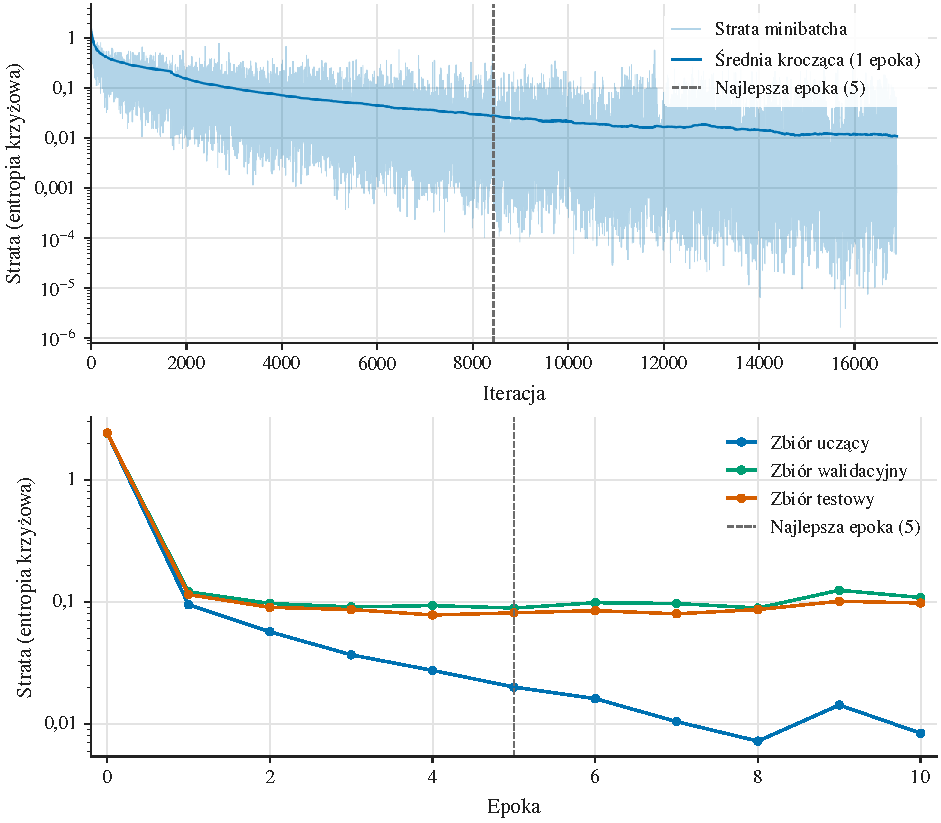
\includegraphics[width=0.9\textwidth]{mnist/final/plots/loss.pdf}
    \caption{Przebieg straty zgłoszonej sieci w skali logarytmicznej. Górny wykres: strata kolejnych paczek i jej średnia krocząca z okna jednej epoki. Dolny wykres: strata na zbiorach uczącym, walidacyjnym i testowym po każdej epoce. Linia przerywana oznacza epokę, z której pochodzi zwrócona sieć.}
    \label{fig:final-loss}
\end{figure}

Macierz pomyłek na zbiorze testowym przedstawiono na Rysunku~\ref{fig:final-confusion}. Najlepiej rozpoznawane są cyfry $0$ i $1$ (\qty{99.39}{\percent} i \qty{99.30}{\percent} poprawnych decyzji), a najsłabiej $4$ (\qty{94.30}{\percent}) i $8$ (\qty{95.69}{\percent}). Najczęstszą pomyłką jest klasyfikacja czwórki jako dziewiątki ($37$ obrazów, \qty{3.8}{\percent} czwórek). Kolejne pomyłki są co najmniej czterokrotnie rzadsze: ósemka jako $9$, $5$ i $3$ (po $9$ obrazów) oraz czwórka jako $7$ ($8$ obrazów).

\begin{figure}[H]
    \centering
    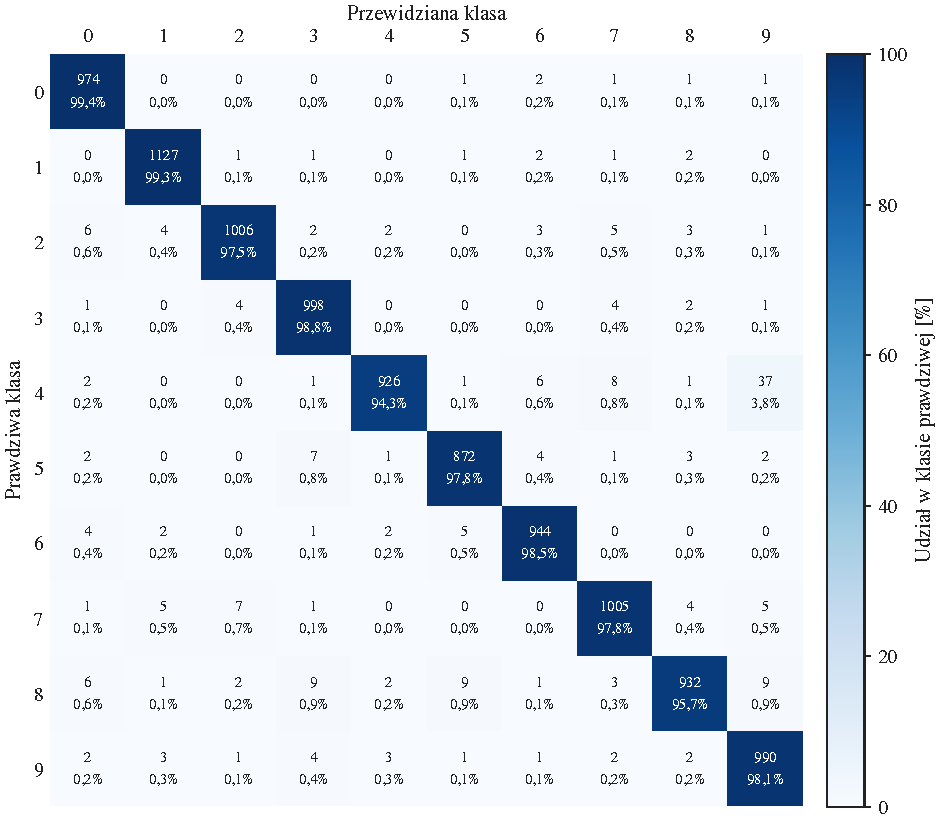
\includegraphics[width=0.75\textwidth]{mnist/final/plots/confusion_test.pdf}
    \caption{Macierz pomyłek zgłoszonej sieci na zbiorze testowym: liczba obrazów i odsetek w wierszu klasy prawdziwej.}
    \label{fig:final-confusion}
\end{figure}

Na Rysunku~\ref{fig:final-misclassified} pokazano $32$ błędnie sklasyfikowane obrazy testowe, którym sieć przypisała największe prawdopodobieństwo błędnej klasy. Spośród $226$ błędów $19$ ma prawdopodobieństwo przewidzianej klasy większe niż \num{0.99}, a $65$ większe niż \num{0.9}. Mediana tego prawdopodobieństwa wynosi dla błędów \num{0.77}. Wśród pokazanych obrazów są cyfry o nietypowym kształcie oraz cyfry przypominające przewidzianą klasę, np. czwórki z zamkniętą górną częścią sklasyfikowane jako $9$.

\begin{figure}[H]
    \centering
    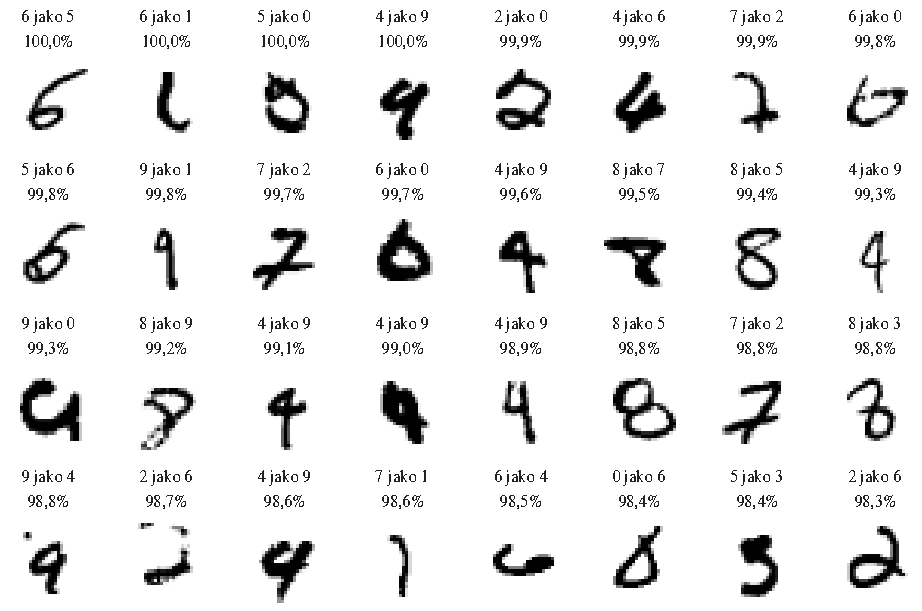
\includegraphics[width=\textwidth]{mnist/final/plots/misclassified.pdf}
    \caption{Błędnie sklasyfikowane obrazy testowe o największym prawdopodobieństwie przewidzianej klasy. Nad obrazem podano klasę prawdziwą, klasę przewidzianą i jej prawdopodobieństwo.}
    \label{fig:final-misclassified}
\end{figure}

Wagi łączące piksele obrazu z pierwszymi $32$ spośród $512$ neuronów warstwy ukrytej przedstawiono jako obrazy $28 \times 28$ na Rysunku~\ref{fig:final-weights}. Część neuronów ma wyraźne, lokalne skupiska wag o jednym znaku, układające się w fragmenty pociągnięć, a u pozostałych wagi nie tworzą widocznej struktury. Szarym kolorem oznaczono $72$ piksele, które mają wartość $0$ we wszystkich \num{54000} obrazach uczących. Zgodnie z podrozdziałem~\ref{sec:problem-dataset} ich wagi nie otrzymują gradientu i pozostają równe wartościom początkowym.

\begin{figure}[H]
    \centering
    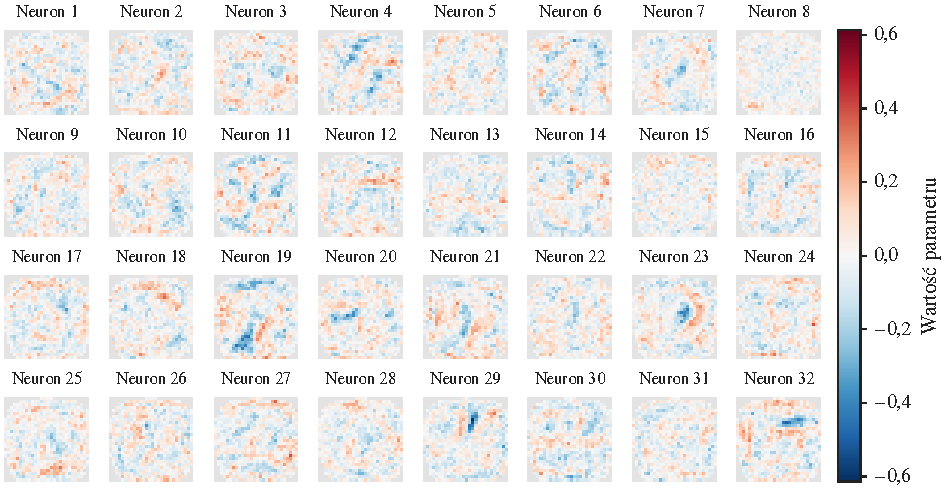
\includegraphics[width=\textwidth]{mnist/final/plots/first_layer_weights.pdf}
    \caption{Wagi pierwszej warstwy zgłoszonej sieci dla pierwszych $32$ neuronów warstwy ukrytej, przedstawione jako obrazy $28 \times 28$ we wspólnej skali barw. Szare piksele są stałe w części uczącej.}
    \label{fig:final-weights}
\end{figure}

\section{Podsumowanie i wnioski}
\label{sec:conclusions}

Perceptron wielowarstwowy z części pierwszej projektu zastosowano do rozpoznawania cyfr MNIST, zmieniając wyłącznie jego parametry. Konfigurację dobrano w pięciu badaniach strojenia na podzbiorze zbioru uczącego, a wybraną konfigurację nauczono na pełnym zbiorze uczącym i oceniono na zbiorze testowym. W rozdziale zebrano najważniejsze wnioski oraz ograniczenia przeprowadzonych badań.

\subsection{Wnioski}
\label{sec:conclusions-findings}

\paragraph{Strojenie}
\begin{itemize}
    \item Liczba neuronów jednej warstwy ukrytej wyraźnie wpływa na wynik: dokładność walidacyjna rośnie z \qty{92.70}{\percent} dla $32$ neuronów do \qty{94.35}{\percent} dla $128$ i \qty{95.16}{\percent} dla $512$. Dodatkowe warstwy ukryte nie poprawiają wyniku względem jednej szerokiej warstwy i zwiększają rozrzut między ziarnami, z odchyleniem standardowym do \num{1.15} punktu procentowego wobec \num{0.39} dla sieci 512 (podrozdział~\ref{sec:tuning-architectures}).
    \item Sieci z ReLU i leaky ReLU osiągają od \num{1.04} do \num{1.15} punktu procentowego większą dokładność walidacyjną niż sieci z funkcją sigmoidalną i tanh, czyli więcej niż rozrzut między ziarnami. Osiągają też minimum straty walidacyjnej w mniejszej liczbie epok (podrozdział~\ref{sec:tuning-activations}).
    \item Normalizacja wejść, optymalizator i rozmiar paczki dają różnice porównywalne z rozrzutem między ziarnami. Wybrane poziomy, czyli normalizacja min-max, Adam z $\eta = \num{0.001}$ i paczka 32, są najlepsze średnio, ale inny zestaw ziaren mógłby wskazać inne (podrozdział~\ref{sec:tuning-summary}).
    \item Standaryzacja nadaje rzadko niezerowym pikselom duże wartości wejść, na części uczącej do około $89$, co jest zgodne z jej słabszym wynikiem od normalizacji min-max (podrozdział~\ref{sec:tuning-normalization}).
\end{itemize}

\paragraph{Sieć końcowa}
\begin{itemize}
    \item Sieć \mbox{784-512-10} z ReLU, normalizacją min-max, optymalizatorem Adam z $\eta = \num{0.001}$ i paczką 32, uczona na pełnym zbiorze uczącym, osiąga na zbiorze testowym \qty{97.91 +- 0.15}{\percent} dla $5$ ziaren. Zgłoszona sieć, z ziarnem ustalonym przed uczeniem, osiąga \qty{97.74}{\percent} (podrozdział~\ref{sec:final-seeds}).
    \item Większy zbiór uczący poprawia wynik tej samej konfiguracji: dokładność walidacyjna rośnie z \qty{95.16}{\percent} przy \num{8000} obrazach uczących do \qty{97.79}{\percent} przy \num{54000}.
    \item Sieć przeucza się także na pełnym zbiorze: dokładność ucząca wynosi \qty{99.33}{\percent}, a strata walidacyjna przestaje maleć po kilku epokach. Wczesne zatrzymanie kończy uczenie po $8$ do $12$ epokach (podrozdział~\ref{sec:final-network}).
    \item Najczęstszą pomyłką zgłoszonej sieci jest klasyfikacja czwórki jako dziewiątki ($37$ z $226$ błędów), a najsłabiej rozpoznawane są cyfry $4$ i $8$.
\end{itemize}

\subsection{Ograniczenia}
\label{sec:conclusions-limitations}

Wnioski obowiązują w warunkach, w których przeprowadzono badania:
\begin{itemize}
    \item każde badanie zmieniało jeden czynnik, a badania przeprowadzono kolejno, więc wybory zależą od kolejności badań i nie wiadomo, czy czynniki na siebie oddziałują, np. czy sieć z funkcją tanh nie wymagałaby innego współczynnika uczenia,
    \item strojenie przeprowadzono na \num{8000} obrazach uczących, a sieć końcową uczono na \num{54000}. Nie sprawdzono, czy przy większym zbiorze uczącym byłyby lepsze inne poziomy, np. głębsze sieci, które na podzbiorze nie przewyższały jednej szerokiej warstwy,
    \item każdy wariant uczono dla $5$ ziaren, a każdy czynnik miał kilka poziomów. Przy różnicach porównywalnych z rozrzutem między ziarnami wybór poziomu jest niepewny, a poziomy spoza badanych siatek, np. inne współczynniki uczenia SGD, nie zostały sprawdzone.
\end{itemize}


%----------------------------------------------------------------------
\newpage
\printbibliography[heading=bibintoc]

%----------------------------------------------------------------------
\appendix
\section{Odtworzenie wyników}
\label{app:reproduction}
% Plan (etap 2): listing final/config.toml, polecenia mnist, train i plot, ziarno 1,
% położenie konfiguracji badań, wersja kodu zapisana w artefaktach.


\end{document}
